\chapter{A functional definition of analogical classifiers}
In recent works, analogy-based classifiers have been proved quite successful.
They exhibit good accuracy rates when compared with standard classification
methods. Nevertheless, a theoretical study of their predictive power has not
been done so far. One of the main barriers has been the lack of functional
definition: analogical learners have only algorithmic definitions.  The aim of
our paper is to complement the empirical studies with a theoretical
perspective. Using a simplified framework, we first provide a concise
functional definition of the output of an analogical learner.  Two versions of
the definition are considered, a strict and a relaxed one.  As far as we know,
this is the first definition of this kind for analogical learner. Then, taking
inspiration from results in $k$-NN studies, we examine some analytic
properties such as convergence and VC-dimension, which are among the basic
markers in terms of machine learning expressiveness. We then look at what could
be expected in terms of theoretical accuracy from such a learner, in a Boolean
setting.  We examine learning curves for artificial domains, providing
experimental results that illustrate our formulas, and empirically validate our
functional definition of analogical classifiers.

\section{Analogical classification}
\label{ANALOGICAL_CLASSIFICATION}
In the context of  classification, items are represented as elements of a universe $X$ having a (unique) label belonging
to $Y$. For any $x\in X$, $\dot{x}$ denotes the ground
truth label associated to $x$. The goal of a classifier is, given a sample
set $S$ (i.e. a set of elements $x \in X$ for which $\dot{x}$ is known), to
correctly predict the label of other elements $x$ that do not belong to the
sample set. We call $\hat{x}$ the predicted label of $x$: this is the output of the classifier.

\subsection{Conservative classifier}
\label{conservative}

Let us first consider what we call a \textit{conservative}
classifier. Such a classifier is called conservative because it
is not able to output a prediction for any $x$ in $X$, but only for a subset of
$X$. We need to define two crucial concepts: the \textit{analogical extension} of
a sample set $S$, and the \textit{analogical root} of an element $x$.

Let $A$ be an analogy relation over $X$ and $B$ an analogy relation over $Y$, the set of labels.
The notion of analogical equation allows us to define the so-called {\it
analogical extension} of $S$ denoted as:
\begin{align*}
  A_E^Y(S)=\{ x \in X | \exists (a,b,c) \in S^3, ~ & a:b::c:x \mbox{ and }\\
& \exists y \in Y, \dot{a}:\dot{b}::\dot{c}:y\}.
\end{align*}
An intuitive interpretation of $A_E^Y(S)$ is to see it as the set of all $x \in
X$ that are solutions of the analogical equations which can be built over the
sample set $S$, provided that the equation related to the associated labels is also solvable.
In the case where $A$ is univocal, if $S$ is finite, then due to the
permutation properties of $A$, $\frac{|S|^3}{2}$ is an upper bound of
$|A_E(S)|$ leading to: $$|S| \leq |A_E(S)| \leq \frac{|S|^3}{2}$$
We have the following properties:
\begin{enumerate}
\item $S \subseteq A_E^Y(S)$, since $x:x::x:x$ always holds~;
\item$A_E^Y(\emptyset)=\emptyset$, $A_E^Y(X)=X$~;
\item $S_1 \subseteq S_2 \implies A_E^Y(S_1) \subseteq A_E^Y(S_2)$.
\end{enumerate}

The dual concept of the analogical extension is the so-called {\it analogical
root} of a given element $x \in X$, denoted $R_{S}^Y(x)$:
$$\quad R_{S}^Y(x) = \{(a, b, c) \in S^3 | a:b::c:x \mbox{ and } \exists
y \in Y, \dot{a}:\dot{b}::\dot{c}:y\}$$
$R_{S}^Y(x)$ is the set of 3-tuples in $S$ which are analogically linked to
$x$ and which provide a prediction for the label. It is clear that $R_{S}^Y(x)$ may contain more than one 3-tuple: for
example in $R^m$, $x$ may be the summit of more than one parallelogram.
$$R_{S}^Y(x) = \emptyset \iff x \notin A_E^Y(S)$$

For any element $x$ of $A_E^Y(S)$, we define the \textit{analogical label} of
$x$ as:
$$\albl{x} = \begin{cases}
\dot{x} \text{ if } x \in S\\
\text{Mode} \{y | \dot{a} : \dot{b} :: \dot{c} : y ~ \forall (a, b, c) \in
R_S^Y(x) \} \text{ if } x \notin S
\end{cases}
$$
where $\text{Mode}(\Sigma)$ returns the most frequent element of the multiset
$\Sigma$. In case of a tie, the returned element is chosen at random between
the most frequent elements.

The analogical label will be used to estimate the label of every element.
Obviously, in the first case, we do not want to change the label of the
elements of $S$.  For elements in $A_E^Y(S) \setminus S$ (i.e.  the second
case), the analogical label is the most frequent label out of all the labels inferred from the
solution of the analogical equations that one can build from $R_S^Y(x)$.  It is
quite clear that, for these elements,  we do not necessarily have
$\albl{x}=\dot{x}$.  To summarize, for a given element $x \in X$, we may 
potentially associate 3 labels:
\begin{itemize}
\item its true label $\dot{x}$~;
\item in the case where $x \in A_E^Y(S)$, its analogical label $\albl{x}$~;
\item its predicted label $\hat{x}$.
\end{itemize}
\noindent
Conservative classifiers set the prediction of an element $x \in A_E^Y(S)$ as
$\hat{x}$ as follows:

$$\mbox{if } x \in A_E^Y(S),  \hat{x} = \albl{x} \mbox{ else } \hat{x} \mbox{ is undefined}$$
This kind of classifier cannot predict a label for an element which is not in $A_E^Y(S)$.
The prediction $\hat{x}$ is not defined if $x$ does not belong to $A_E^Y(S)$.
In Algorithm \ref{algo_conserv}, we provide the corresponding algorithm.

\begin{algorithm}[!ht]
 \caption{\textit{Conservative classifier}}
       \label{algo_conserv}
       \begin{algorithmic}

      \STATE {\bf Input}: A sample set $S$ and an element $x \in X$ for which
      $\dot{x}$ is unknown.
      \STATE {\bf Output}: $\hat{x}$, an estimation of $\dot{x}$
      \STATE {\bf Init}: $C = \varnothing$ \quad \quad // multiset of candidate labels

      \FORALL{$(a, b, c) \in S^3$ such that $a : b :: c : x$}
      \IF{$\exists y \in Y$ such that $\dot{a} :\dot{b} ::\dot{c} : y$}
      \STATE // we are sure $(a, b, c) \in R_S^Y(x)$
      \STATE compute the solution $y$ of $\dot{a} : \dot{b} : \dot{c} : y$
      \STATE $ C = C \cup y$
      \ENDIF
	    \ENDFOR
      \STATE $\hat{x} = \albl{x}  = \text{Mode} (C)$ // undefined if $C = \varnothing$
\end{algorithmic}
\end{algorithm}

\paragraph{Algorithm}
\begin{itemize}
\item Compute $A_E^Y(S)$.
\item If $x \notin  A_E^Y(S)$, $x$ is not classifiable.
\item If $x \in  A_E^Y(S)$, for each $a,b,c \in R_{S}^Y(x)$ compute
the solution of the equation $\dot{a}:\dot{b}::\dot{c}:y$.
\item Predict $\hat{x}$ as the majority label among the previous solutions.
\end{itemize}
Let us note that $A_E^Y(S)$ is never explicitly computed. Instead, we look for
every 3-tuple in $S$ and check if they belong to $R_S^Y(x)$.
Clearly, this is a supervised learning setting, where sample instances are
stored for future use, without any generalization process. Conservative
classifiers are Instance Based Learners
as described in \cite{Aggar2014}.
Therefore, analogical learner ranges among the category of Instance Based Learners.

Let us sketch an example coming from
\cite{StrYvoReport2005} where an analogical relation is defined on the set of
words over a finite alphabet. The learning task is to learn the conjugation of
English verbs. Solving the analogical equation $view:reviewer::search:y$ leads
to $researcher$, using the definition of the analogy and the concatenation
operator. Similarly given a sample set $S=\{x_1,x_2,x_3,x_4,x_5\}$ where

$x_1=(read,3,reads), x_2=(read,G,reading), x_3=(view,3,views)$,

$x_4=(view,G,viewing), x_5=(eat,3,eats)$

and a new element $x=(eat,G,y)$, then $R_S^Y(x)= \{(x_1,x_2,x_5),
(x_3,x_4,x_5)\}$. The prediction is $\hat{x}=eating$ which is the solution of
the equation $view:viewing::eat:y$. And this is exactly what is expected.  But
there is no solution for $x=(absurd,G,y)$ just because $R_S^Y(x)= \emptyset$.

Such a conservative learner cannot generalize to any new input and is
restricted to elements in $A_E^Y(S)$. This is not the case for instance-based
learner like $k$-NN.  This is why other options have been implemented to
overcome this problem and to extend in some sense the generalization ability of
analogical learner, as we will see in the next section.

\subsection{Extended classifier}
\label{EXTENDED_LEARNER}

To relax the previous option, we need to be able to predict a label for
elements outside $A_E^Y(S)$ i.e. elements which do not constitute a perfect analogy
with elements in $S$.  To this end, we can try to measure to what extent such
elements are far from building a perfect analogy with those in $S$.
The concept of {\it analogical dissimilarity}, first  defined in
\cite{BayMicDel2007}, will be useful to  quantify in some sense how far a
relation $a:b::c:d$ is from being a valid analogy.
We keep the initial notation $AD(a,b,c,d)$ to
denote the analogical dissimilarity between 4 elements.  Some  minimal
properties have to be satisfied by such a dissimilarity $AD: X^4 \longrightarrow \mathbb{R}^+$ to fit with the intuition:
\begin{itemize}
\item $\forall a, b, c, d, \quad  AD(a,b,c,d)=0 \mbox{ iff } a:b::c:d$
\item $\forall a, b, c, d, \quad  AD(a,b,c,d)=AD(c,d,a,b)=AD(a,c,b,d)$
\item $\forall a, b, c, d, e, f,  AD(a,b,e,f) \leq AD(a,b,c,d) + AD(c,d,e,f)$
\end{itemize}
As the definition of an analogy strongly relies on the structure and operators
available on $X$, we have the same situation for $AD$: there are a lot of
possibilities. For instance:
\begin{itemize}
\item When $X=\mathbb{R}^m$ and $a:b::c:d \mbox{ iff } a-b=c-d$, $AD(a,b,c,d) =
  ||(a-b)-(c-d)||_p$ is an analogical dissimilarity for any $p$,
  where $||.||_p$ denotes the standard $p$ norm  in $\mathbb{R}^m$.
\item
When $X=\mathbb{B}$ and $a:b::c:d \mbox{ iff } (a \wedge b \equiv c
  \wedge d) \wedge (a \vee  b) \equiv (c \vee d)$, one can define an analogical
  dissimilarity $AD(a,b,c,d)$ as the number of values that have to be switched
  to get a proper analogy. For instance, $AD(0,1,0,0)=1$ and $AD(0,1,1,0)=2$.
The codomain of $AD$ is just $\{0, 1, 2\}$. When extended to
  $X=\mathbb{B}^m$ with $$AD(a,b,c,d) = \sum\limits_{i=1}^m AD(a_i,b_i,c_i,d_i),$$
  we get an analogical dissimilarity whose co-domain is $[0, 2m]$. In fact,
  this definition is just the restriction to $\mathbb{B}^m$ of the one coming
  from $\mathbb{R}^m$, when considering that $\mathbb{B}^m \subseteq
  \mathbb{R}^m$ and using the $L_1$ norm, i.e. $AD(a,b,c,d) = ||(a-b)-(c-d)||_1$.
\end{itemize}

As a measure of \textit{how poorly an analogical proportion holds}, the
analogical dissimilarity will help to define more flexible classifiers.  The
main underlying idea is to consider {\it approximate} analogies which are not
valid stricto sensu, but not too far to be valid.
In \cite{BayMicDel2007}, after defining analogical dissimilarity,  the authors
build an extended classifier allowing classification of elements that do not
belong to $A_E^Y(S)$.  Algorithm \ref{algo_extended} gives a description of
their classifier.
\begin{algorithm}[!ht]
 \caption{\textit{Extended classifier}}
       \label{algo_extended}
       \begin{algorithmic}

      \STATE {\bf Input}: A sample set $S$, an element $x \in X$ for which
      $\dot{x}$ is unknown, a constant $k$.
      \STATE {\bf Output}: $\hat{x}$, an estimation of $\dot{x}$
      \STATE {\bf Init}: $C = \varnothing$ \quad \quad // multiset of candidate labels
      \FORALL{$(a, b, c) \in S^3$ such that $\exists y \in Y$ with $\dot{a} :\dot{b} ::\dot{c} : y$}
        \STATE compute $AD(a, b, c, x)$ and store it
	    \ENDFOR
      \FORALL{$k$ least values of $AD(a, b, c, x)$}
      \STATE compute the solution $y$ of $\dot{a} : \dot{b} : \dot{c} : y$
      \STATE $C = C \cup y$
    \ENDFOR
    \STATE $\hat{x} = \text{Mode}(C)$
\end{algorithmic}
\end{algorithm}

This algorithm is similar to the conservative one but, instead of looking for
pure analogies, we allow for some analogies not to be perfect when we need to.
In their implementation \cite{BayMicDel2007}, the authors actually look for
all the 3-tuples that have the same analogical dissimilarity as the $k$th one:
this allows them to fit with the previous conservative approach. For the sake of
simplicity, we have chosen to
ignore this small detail in our explanation.

In \cite{BayMicDel2007}, the authors evaluated this classifier on a Boolean setting
$\mathbb{B}^m$ over 8 benchmarks from the UCI repository.  This approach led to
remarkable results in terms of accuracy, when compared to off-the-shelf
standard classifiers.

Nonetheless, this algorithm does not allow us to grasp its inherent working
behaviour and it is difficult to extract theoretical properties. The aim of the
next subsection is to give a functional translation of this algorithmic
description.


\subsection{Analogical classifier: a functional definition}\label{FUNCTIONAL_DEF}

As we have seen in the previous section, in the case of a Boolean setting,
$AD(a,b,c,d)= ||(a-b)-(c-d)||_1$.  A simple rewriting leads to:
$$AD(a,b,c,d)=||d - (c-a+b)||_1=||d - d'||_1,$$
where $d'=c-a+b$. Actually, $d'$ is nothing but the 4th vertex of the
parallelogram $abcd'$ so this means that $AD(a,b,c,d)$ simply is the $L_1$ distance
 from $d$ to this 4th vertex. Note that as $\mathbb{B}^m$ is not closed for
addition, $d'$ might not belong to $\mathbb{B}^m$ but to $\mathbb{R}^m$: this
happens when one of the terms $AD(a_i, b_i, c_i, d_i)$ is equal to $2$, as
further discussed later.

As we have seen, for a given $x \in X$, algorithm \ref{algo_extended} tries to
minimise $AD(a,b,c,x)$ over all the 3-tuples $(a,b,c) \in S^3$. In the
light of what has just been explained, we see that this is equivalent to
finding the closest vertex $d'=c-a+b$  from $x$ for any $(a, b, c) \in S^3$.


Denoting $\delta$ the $L_1$ distance, $AD(a,b,c,d) =\delta(a-b,c-d) =
\delta(d,d')$,
In the case where $k=1$, the
works of \cite{BayMicDel2007} will predict $\hat{x}$ as the label $\dot{d'}$ of
this summit $d'$. \todo{verifier. C'etait en comm}
it is then natural to consider what we call the \textit{nearest analogical
neighbour} (or \textbf{nan}) of $x$ from a sample $S$ as the element of
$A_E^Y(S)$ defined as:
$$\forall x \in X, \forall S \subseteq X, 1\mbox{-nan}(x,S)\eqdef \argmin_{d'
\in A_E^Y(S)} \delta(x,d')$$
When there is more than one nan, one can either proceed to a majority vote
procedure among all their analogical labels, or randomly select one of these.
This last option is the one we chose in our implementation.
\begin{property} \label{propnn}We have the following equality:
$$1\mbox{-nan}(x,S)= 1\mbox{-nn}(x,A_E^Y(S)).$$
\end{property}
The analogical classification rule simply is:
$$\hat{x} = \albl{1\mbox{-nan}(x,S)}.$$
In words, the predicted label of an element $x$ is the analogical label of its
nearest neighbour in $A_E^Y(S)$.
In some sense, an analogical classifier behaves
as a $\NN$ classifier but on an extended sample set.

Obviously if $x$ belongs to $A_E^Y(S)$ then $x$ is its own nearest analogical
neighbour: $\nan(x, S) = x \text{ iff } x \in A_E^Y(S)$. Therefore, it is easy
to see that this rule is a generalisation of the conservative approach.
Instead of using only one nearest analogical neighbour, we can consider the set
of the $k$ nearest analogical neighbours, and implement a majority vote as it is
done in \cite{MicBayDelJAIR2008}.

The above definition leads to understand the process of analogical classification as follows:
\begin{enumerate}
  \item First, extend the sample set $S$ to its analogical extension
    $A_E^Y(S)$. $A_E^Y(S)$ can be viewed as an extended sample set that has
    \textbf{class noise}: the label associated with elements in $A_E^Y(S)
    \setminus S$ is their analogical label (as defined in \ref{conservative}),
    which may not be correct.
  \item Then just apply a classical $k$-NN strategy over this extended sample
    set.
\end{enumerate}

Figure \ref{extension} gives an illustration of the classification process: the
label of $x \in X$ is unknown, and we set it to that of $d' \in A_E^Y(S)$ (a
circle), which is its nearest analogical neighbour. To show that the analogical
label of $d'$ has itself been inferred, it is depicted as transparent instead of
plain black.
\begin{figure}
\caption{A graphical view of $A_E^Y(S)$ and the classification process.}
\label{extension}
\begin{center}
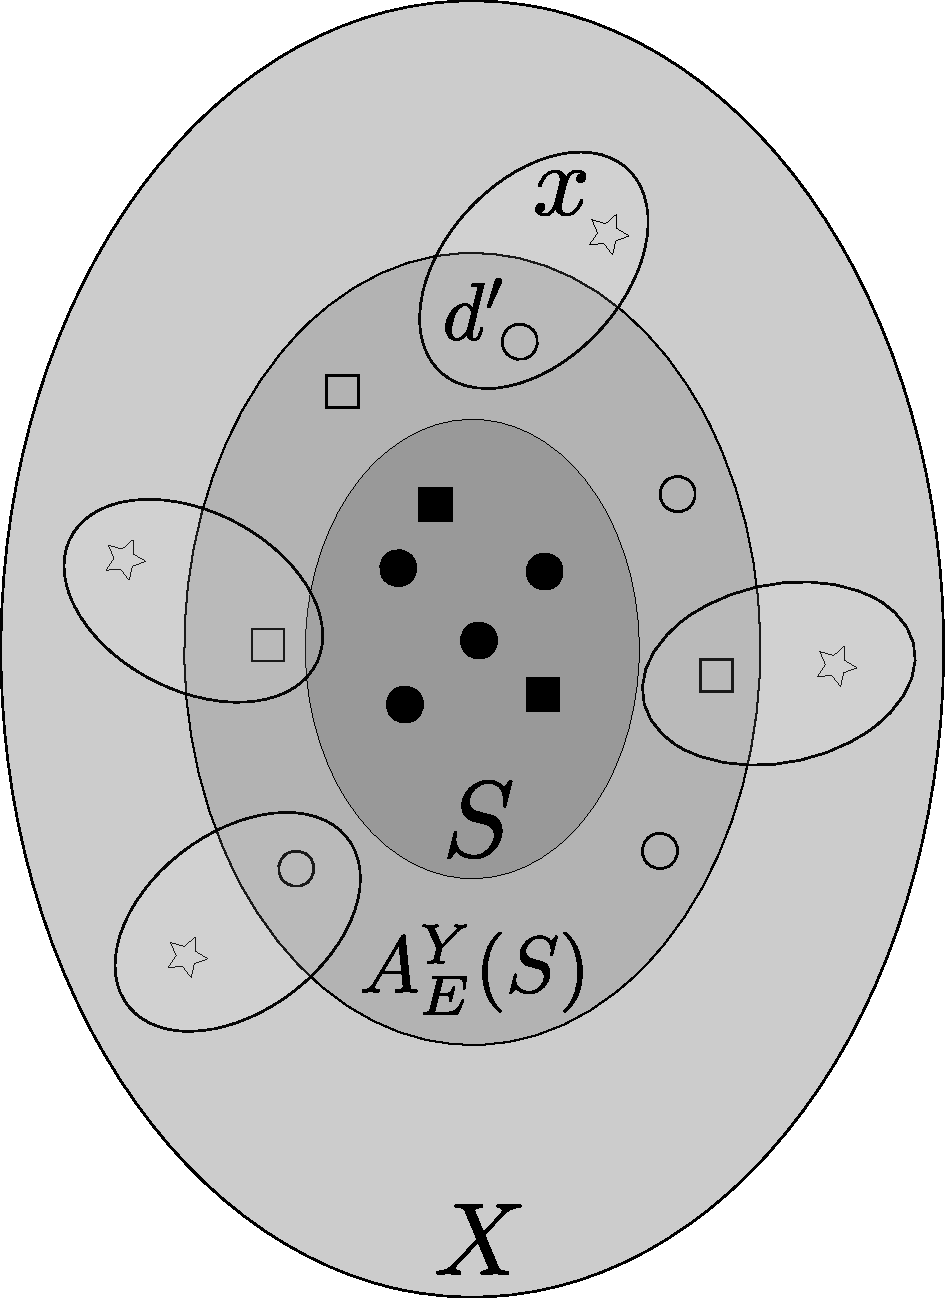
\includegraphics[scale=0.20]{figures/analogical_extension.pdf}
\end{center}
\end{figure}
Let us note that topologically speaking, Figure \ref{extension} is not
representative of a real case: even if we always have $S \subseteq A_E^Y(S) \subseteq X$,

this does not mean that these sets are embedded into one another as shown in
the drawing. Actually, elements of $S$ (and thus of $A_E^Y(S)$) are usually
scattered over the whole universe.

As far as we know, this is the first time a functional definition of
analogy-based classifiers is given. This definition clearly fits with the known
algorithms but obviously, some implementation details cannot be exactly caught
up by such a high level description. It is indeed possible to find a few edge
cases where this functional definition may not output the same result as
algorithm \ref{algo_extended}: this is the case for example when the nan of $x$
is not unique. It is
also the case when the closest vertex $d'$ does not belong to $B^m$.  However,
as we will see in Section \ref{validation} these cases are not likely to occur
and both approaches produce very similar results, thus empirically validating
this functional definition.

Since we now have a clear functional definition of analogical classifiers, we
are in position to examine some general properties such as convergence and
VC-dimension of analogical learners. This is the purpose of the next section.

\section{Some properties in the real case}\label{convergence}
Let us consider the case where $X=\mathbb{R}^m$, $\delta$ any distance issued
from a norm, $AD(a,b,c,d)=\delta(a-b,c-d)$ and $x \in X$.  In any case, just
because $S \subseteq A_E(S)$, we have the following inequality:
$$\delta(x, \nan(x,S)) \leq \delta(x, \nn(x,S))$$

\subsection{Study of convergence}

Now, let us consider  $x^{(i)}$ an i.i.d. sequence of random variables in
$\mathbb{R}^m$, where $\mathbb{R}^m$ is equipped with a probability measure
denoted $P$. As the set $S_n=\{x^{(i)}, ~ i \in [1, n]\}$ is random, then
$\nan(x,S_n)$ can also be considered as a random element of $X$.  We then are
in the exactly same context as the work of Cover \& Hart (\cite{CovHar1967}), and
we obtain the same result:
\begin{property}\label{propconvergence}
$plim_{n \to \infty}(\nan(x,S_n))=x$ almost surely,
\end{property}
where $plim$ is the probability limit operator.

{\it Proof}:
Exactly the same proof  as in \cite{CovHar1967} could be applied.  But it is
simpler to remember that $\delta(x, \nan(x,S_n)) \leq \delta(x, \nn(x,S_n))$. Then,
for a given $x$, the convergence in probability of $\delta(x,
\nn(x,S_n))$ to $0$ implies the convergence in probability of $\delta(x,
\nan(x,S_n))$ to $0$ which exactly means what needs to be proven.
The subset of $X$ where $plim_{n \to \infty}(\nan(x,S_n))\neq
x$ is included into the subset of $X$ where $plim_{n \to \infty}(\nn(x,S))\neq x$:
Cover \& Hart lemma tells us that this set has probability $0$. Thus the final
result.\hfill $\blacksquare$\\

Let us note the following points:
\begin{enumerate}
\item The lemma of Cover and Hart is more general than the one above. They have
  proven the result for any separable metric space, without any additional
  information. In fact, we cannot follow these lines here just because there is
  no known way to define an analogical dissimilarity on a metric space, without
  the help of other structure or operator (see \cite{MicBayDelJAIR2008} for a
  detailed discussion on this issue).
\item This result does not say anything regarding the prediction accuracy of
  $1\mbox{-nan}$ prediction rule as it is rather different than the
  $1\mbox{-nn}$ rule. Such consideration will be investigated in Section
  \ref{accuracy}.
\item We have to be careful about the interpretation of this property in terms
  of machine learning. Indeed, a stronger property is proved in
  \cite{CovHar1967}: for an {\it integrable} function $f$  over $\mathbb{R}^m$
  w.r.t. the probability measure $P$, the expectation of
  $f(\nn(x,S_n))- f(x)$ converges to 0 when $n$ goes to infinity.
  This means that asymptotically, the nearest neighbour of $x$ has the same
  properties as $x$, and then the same label. Such a property has not yet been
  proven for $\nan(x, S_n)$.
  For instance $\mathbb{B}^m$, when considered as a finite
  subset of $\mathbb{R}^m$ and equipped with the metric topology resulting from
  $\mathbb{R}^m$, is a separable metric space (because it is finite).
  Therefore, property \ref{propconvergence} still holds and actually even the
  Cover \& Hart lemma holds). However, this does not mean that for a given
  element $x$ the characteristics (i.e. the labels) of its nearest analogical
  neighbour converge to $\dot{x}$
\item Finally, it is clear that when $n$ goes to infinity, the behavior of an
  analogical classifier tends to that of a nearest neighbours classifier.
  Indeed, when $S_n$ is very big, the nearest analogical neighbour of an
  element $x$ simply is its nearest neighbour, in most cases. Moreover, when
  the nan and the nn are too close, paying the price of the noise related to
  the nan may not be worth it. This supports the common acknowledgement that
  analogical reasoning is mostly useful when very few data are available.
    In this later case extending a small sample set with its analogical
    extension may be particularly beneficial.



\end{enumerate}
To conclude this discussion, even if the convergence result is interesting in
itself, it does not say a lot in terms of machine learning.

To summarize, an analogical classifier extends the sample set $S$ into its
analogical extension $A_E^Y(S)$, then applies the $1\mbox{-nn}$ rule. A
fundamental difference is that the set $A_E^Y(S)$ is also made of elements
whose label is predicted and is not 100\% sure.

\subsection{VC-dimension}\label{vcdim}
The notion of VC-dimension was originally defined by Vapnik and Chervonenkis \cite{Vapnik1998}, and introduced into learnability theory by Blumer et al. \cite{Blumer1989}. Roughly speaking, the VC-dimension of a class of learners is a numerical measure of their discrimination power. It appears that this number is strongly linked to the confidence interval between the empirical risk (i.e. the error a learner makes on the sample set) and the true risk (the error a learner makes on the whole universe $X$). As such, the VC-dimension of a class of learners is an essential element of their theoretical study.
We consider a universe $X$ (usually a Cartesian product to represent the data) and a
family $\mathcal{H}=\{h_i \subseteq X|i \in I\}$ of subsets of $X$.
The elements of $\mathcal{H}$ will be referred as hypothesis or models.
Given a subset $A$
of $X$, we can consider the new family of subsets $tr(\mathcal{H},A) = \{h_i \cap A \subseteq X|i \in I\}$: this family is called the {\it trace of $\mathcal{H}$ over $A$}. This is obviously a subset
of the power set of $A$, $2^A$ i.e. $tr(\mathcal{H},A) \subseteq 2^A$.
We say that $\mathcal{H}$ shatters $A$ iff $tr(\mathcal{H},A)=2^A$.
$VC\mbox{-}dim(\mathcal{H})$ is then the size of the largest finite subset which can be shattered by $\mathcal{H}$:
\begin{definition}
  $VC\mbox{-}dim(\mathcal{H}) = \bigsqcup \{|A| \given[\big] \mathcal{H} \mbox{ shatters } A
\}$,
\end{definition}
where $\bigsqcup$ is the least upper bound operator.
In the case where $\forall n \in\mathbb{N}, \exists  A \subset X, |A|=n \mbox{ such
that } \mathcal{H} \mbox{ shatters } A$, we simply say that:
$$VC\mbox{-}dim(\mathcal{H})=\infty.$$
\noindent
As a binary classifier $c$ over $X$ defines a subset of $X$ with $c^{-1}(1)=\{x \in X | c(x)=1\}$, we can associate to a class $\mathcal{C}$ of classifiers a family of subsets
$\{c^{-1}(1) | c \in \mathcal{C}\}$ and then the $VC\mbox{-}$dimension of a set of classifiers is as below:
\begin{definition}
$VC\mbox{-}dim(\mathcal{C})=VC\mbox{-}dim(\{c^{-1}(1) | c \in \mathcal{C}\})$
\end{definition}
For instance with $X=\mathbb{R}^n$ and with $\mathcal{C}$ the family of the $k$-NN
classifiers: $\mathcal{C}_{\text{NN}}=\{ k\text{-NN classifiers}, k \in \mathbb{N}^*\}$,
then $VC\mbox{-}dim(\mathcal{C}_{\text{NN}})=\infty$.
Let us now consider the family of analogical binary classifiers $\mathcal{AC}_k$ whose classification rule is as below (where a majority vote is implemented):
$$\mathcal{AC}_k(x,S) = \albl{k\mbox{-}nan(x,S)}$$
In view of the previous section, $VC\mbox{-}dim(\mathcal{AC}_k)$ is clearly defined and has to be computed
or at least estimated.
In fact, an immediate result comes, derived from the core definition of an analogical proportion:
\begin{property}\label{vcdimprop}
$VC\mbox{-}dim(\mathcal{AC}_k) = \infty$
\end{property}
{\it Proof}: Given any $x$, the analogical proportion $x:x::x:x$ always
holds so that $\nan(x,S)=x$ then the label $\hat{x}$ allocated to $x$ by $AC_1$
is just $\albl{x}$, which by definition equals $\dot{x}$. It means any set of items can be
exactly labelled, thus the infinite $VC\mbox{-}dim$.  \hfill $\blacksquare$\\
Regarding Property \ref{vcdimprop}, the $\mathcal{AC}_k$ class
behaves exactly as the $k\mbox{-NN}$ class.
Let us note that this is a very general result, which does not rely on any definition of distance.
This is directly coming from a core property of analogical proportions.

\section{Accuracy analysis in the Boolean case}\label{accuracy}

In this section, we study the accuracy of an analogical classifier, and more
particularly that of the $1$-nan classifier ($\NaN$). To do so, we restrict
our view to a Boolean setting: elements to be classified belong to
$X=\mathbb{B}^m$ and the label space is $Y = \mathbb{B}$.

As explained in Section \ref{FUNCTIONAL_DEF}, for a given $x \in X$ and a sample set
$S \subset X$, we have:
\begin{equation}\label{eq1}
\hat{x}=\albl{\nan(x, S)}=\albl{\nn(x, A_E^Y(S))},
\end{equation}
where $A_E^Y(S)$ is the analogical extension of $S$, that we will simply denote
by $A_E$ in what follows for notational brevity.  We also denote $A_E^*
\eqdef A_E \setminus S$ as the set of elements that belong $A_E$ but not to
$S$.

We now equip the set $X$ with a probability distribution denoted $P$.  The
accuracy of the $\NaN_S$ classifier\footnote{The $S$ subscript is here to
  specify that the training set of the $\NaN$ algorithm is $S$. The same
  notation is used for the \textit{nearest neighbour} algorithm: $\NN_\Sigma$ is the
  $\NN$ algorithm trained on the set $\Sigma$.} over all the elements of $X$ is
  defined as: $$\acc(\NaN_S, X)\eqdef P(\hat{x}=\dot{x} \given[\big] x \in X)$$ By
  observing that for any $x$, its $\nan$ either belongs to $S$ or to $A_E^*$,
  the above equation can be split into two distinct parts as follows:

  \begin{align*}
  &P\left(\hat{x}=\dot{x} \given[\big] x \in X\right) = P\left(\albl{\nan(x,
  S)} = \dot{x}\right)\\
=~&P\left([\albl{\nan(x, S)} = \dot{x} ]\wedge [\nan(x, S) \in S
] \right)~ + \\
&P\left([\albl{\nan(x, S)} = \dot{x}] \wedge [\nan(x, S) \in A_E^*]\right)\\ \mbox{(law of total probability)}\\
=~&P\left([\albl{\nn(x, A_E)} = \dot{x}] \wedge [\nn(x, A_E) \in S ]\right)~ + \\
  &P\left([\albl{\nn(x, A_E)} = \dot{x}] \wedge [\nn(x, A_E) \in A_E^*]\right)
\\
=~&P\left([\albl{\nn(x, A_E)} = \dot{x}] \given[\big] [\nn(x, A_E) \in S
]\right) \times \\ &P\left([\nn(x, A_E) \in S]\right) ~+ \\
&P\left([\albl{\nn(x, A_E)} = \dot{x}] \given[\big] [\nn(x, A_E) \in
A_E^*]\right) \times \\ &P\left([ \nn(x, A_E) \in A_E^*]\right)
\end{align*}

Let us denote  $\alpha \eqdef P(\nn(x, A_E) \in S)$\footnote{Obviously, we
also have $\alpha = P(\nan(x, S) \in S)$.}.
The formula becomes:
\begin{align*}
  &\acc(\NaN_S, X) = \\&P\left([\albl{\nn(x, A_E)} = \dot{x}] \given[\big] [\nn(x, A_E)
\in S] \right) * \alpha ~+ \\
&P\left([\albl{\nn(x, A_E)} = \dot{x}] \given[\big] [\nn(x, A_E) \in
A_E^*]\right) * (1 -
\alpha).
\end{align*}

Let us focus on the first term  (discarding the factor $\alpha$):
$$P\left([\albl{\nn(x, A_E)} = \dot{x}] \given[\big] [\nn(x, A_E) \in S] \right)$$

It is easy to see that the event $[\nn(x, A_E) \in S]$ is equivalent to
the event $[\nn(x, A_E) = \nn(x, S)]$. As a result, we can transform the first
term to get a better grasp of its meaning:
\begin{align*}
  &P\left([\albl{\nn(x, A_E)} = \dot{x}] \given[\big] [\nn(x, A_E) \in S] \right)\\
  =~ &P\left([\albl{\nn(x, A_E)} = \dot{x}] \given[\big] [\nn(x, A_E) = \nn(x,
  S)]\right)\\
  =~ &P\left([\albl{\nn(x, S)} = \dot{x}] \given[\big] [\nn(x, A_E) \in S]\right).
\end{align*}

In this form, the first term is just the accuracy of the $\NN_S$ algorithm over
the elements that have their nearest analogical neighbour in $S$.
As for the second term, the same process can be applied by observing that the
event $[\nn(x, A_E) \in A_E^*]$ is equivalent to the event $[\nn(x, A_E) = \nn(x,
A_E^*)]$. This leads to
\begin{align*}
  &P\left([\albl{\nn(x, A_E)} = \dot{x}] \given[\big] [\nn(x, A_E) \in
A_E^*]\right)\\
  =~ &P\left([\albl{\nn(x, A_E^*)} = \dot{x}] \given[\big] [\nn(x, A_E) \in
A_E^*]\right).
\end{align*}

This second term is then the accuracy of the $\NN_{A_E^*}$ algorithm over the elements
that have their nearest analogical neighbour in $A_E^*$.

In the light of these interpretations, one can rewrite the accuracy formula in
a  concise form, using a few more definitions:
\begin{itemize}
\item $A \eqdef \{x \in X, \nan(x, S) \in S\}$: the elements that have
  their nan in $S$.
\item $B \eqdef \{x \in X, \nan(x, S) \in A_E^*\}$: the elements that have
  their nan in $A_E^*$.
\end{itemize}

Naturally, $A \cup B = X$ and $A \cap B = \emptyset$. Also, $\alpha = P(x \in
A)$ and $1 - \alpha = P(x \in B)$. Therefore, the accuracy of $\NaN_S$ over $X$
can be understood as the weighted sum of the accuracy of $\NN$ over $A$ and
$B$, using a different sample set each time (respectively $S$ and $A_E^*$):
\begin{align*}
  \acc(\NaN_S, X) = ~&\acc(\NN_S, A) \cdot \alpha ~ + \\
                    &\acc(\NN_{A_E^*}, B) \cdot (1 -
  \alpha).\numberthis\label{ACCURACY_FORMULA}
\end{align*}
The value $\acc(\NN_S, A)$ is the accuracy of $\NN_S$ over all the elements in
$A$. A theoretical study of this accuracy has been done in
\cite{LanIbaIJCAI1993} when the size of $A$ is known.  Regarding
$\acc(\NN_{A_E^*}, B)$, this is the accuracy of $1$-nn when the sample set is
noisy, and has been studied in \cite{OkaYugIJCAI1997}. This last formula leads
to the consistent facts:
\begin{enumerate}
\item The smaller $A_E^*$ (i.e. analogical reasoning does not
  bring much more labels), the closer $\alpha$ is to $1$, the closer $A$ is to
  $X$ and the more the accuracy of $\NaN_S$ tends towards the accuracy of
  $\NN_S$ over $X$.
\item In return, if $A_E$ is much bigger than $S$, $\alpha$ is then small, $B$
  is close to $X$ and the accuracy of $\NaN_S$ greatly depends on the quality
  of $A_E$, which can be measured by the value $\omega$ defined as: $$\omega
  \triangleq P(\albl{x} = \dot{x} \given[\big] x \in A_E^*).$$ Note that the
  value $1 - \omega$ corresponds to the class noise of $A_E$. As we will see in
  the next section, this situation where $A_E$ is big with respect to $S$ is
  actually extremely likely to occur.
  \end{enumerate}
\section{Experiments and empirical validation}
\label{validation}
In order to get an empirical validation of our formulas, we have developed a set of
experiments that we describe in the next subsection.
\subsection{Validation protocol}
Working with Boolean vectors, we have computed the accuracies of the $\NaN$ and
$\NN$ algorithms over $X=\mathbb{B}^m$ for different values of $m$ (namely $8$
and $10$). The ground truth label of elements of $X$ is
defined by different Boolean functions $f$ in such a way that the $\forall x =
(x_1, \cdots, x_m), ~ \dot{x} = f(x)$. The different functions we have worked
with are:
\begin{itemize}
\item $f(x)=x_m$: in that case, we can consider the $m-1$ first
  parameters are a kind of noise since they have no influence on the final
  label ;
\item $f(x) = 1 \mbox{ iff at least } l  \mbox{ components are equal
  to } 1$ (this kind of function is usually called $l\text{-of-}m$). We chose
  to set $l$ to $\frac{m}{2}$ ;
\item $f(x)= x_1 \oplus  x_2$ (xor): we here have $m-2$ useless attributes ;
\item $f(x)=1 \mbox { iff } \sum x_i =2$: all the attributes are relevant in
  that case~;
\item $f(x)=1 \mbox { iff } \sum x_i = m-1$: an extreme case of
  the previous one~;
\item $f(x)=1 \mbox { iff } x_1 \cdot x_m = 1$: only the first and
  the last elements are relevant.
\end{itemize}

Regarding the size of the training set, to be sure to fit with the size of the
universe, we have investigated various sizes between $3$ and $100$. When
dealing with a training set of size $100$, the cubic complexity of the
analogical classifier leads to explore a set of approximately $100^3$ elements:
as a consequence, we limit our investigation to a maximum of 100 elements in
the training set in order to get realistic execution time.

All the accuracy (and other metrics) computations are averaged over a set of
$100$ experiments.  The interested reader may find the Python source code that
has generated all our plots and detailed results on
Github\footnote{https://github.com/Niourf/nan\_study}. For lack of space,
we only provide a few examples which are representative of the global behavior.
Please note that our implementation of the $\NaN$ algorithm is not that of
algorithm \ref{algo_extended}, but is instead that of the functional definition
of the analogical classifier developed in Section \ref{FUNCTIONAL_DEF}: we
first construct the analogical extension set of $S$, and then proceed to a
nearest neighbour strategy over this noisy extended training set. We have
estimated probabilities by frequencies, thus implicitly assuming a uniform
distribution on $X$.

In addition to these Boolean functions, we have also run the $\NaN$ algorithm
over the Monk datasets over the UCI
repository\footnote{https://archive.ics.uci.edu/ml/datasets/MONK's+Problems}.
They are datasets of 432 binarized elements, among which exactly 169 of them
have been used for training.

\subsection{Experiments}

Figure \ref{plots} shows the accuracies (left column) of the $\NaN$ and $\NN$
over six different Boolean settings with values of $|S|$ varying from $3$ to
$100$. In the right column, we have plotted three different values that will
help us analyse and validate the behaviour of the
$\NaN$ algorithm:
\begin{itemize}
  \item the theoretical accuracy as defined by equation
    (\ref{ACCURACY_FORMULA})
    in Section \ref{accuracy}. The probability $\alpha = P(x \in A$) has been
    estimated by the frequency:~$\frac{|A|}{|X|}$~;
  \item the quality of $A_E^Y(S)$, measured by $\omega$ as defined in Section
    \ref{accuracy} which is estimated by the frequency:~$\frac{|\{x \in A_E^*
    \given[\big] \albl{x} = \dot{x}\}|}{|A_E^*|}$~;
\item finally, the
    quantity $\gamma = \frac{|A_E^Y(S)|}{|X|}$: the size of
    the analogical extension set with respect to that of the whole universe.
\end{itemize}

\begin{figure}[h!]
\caption{Accuracies of the $\NaN$ and $\NN$ algorithms  over different Boolean
  settings and training set sizes, with corresponding values of $\omega$,
  $\gamma$, and theoretical accuracy. The $x$ axis corresponds to the size of
the training set.}
\label{plots}
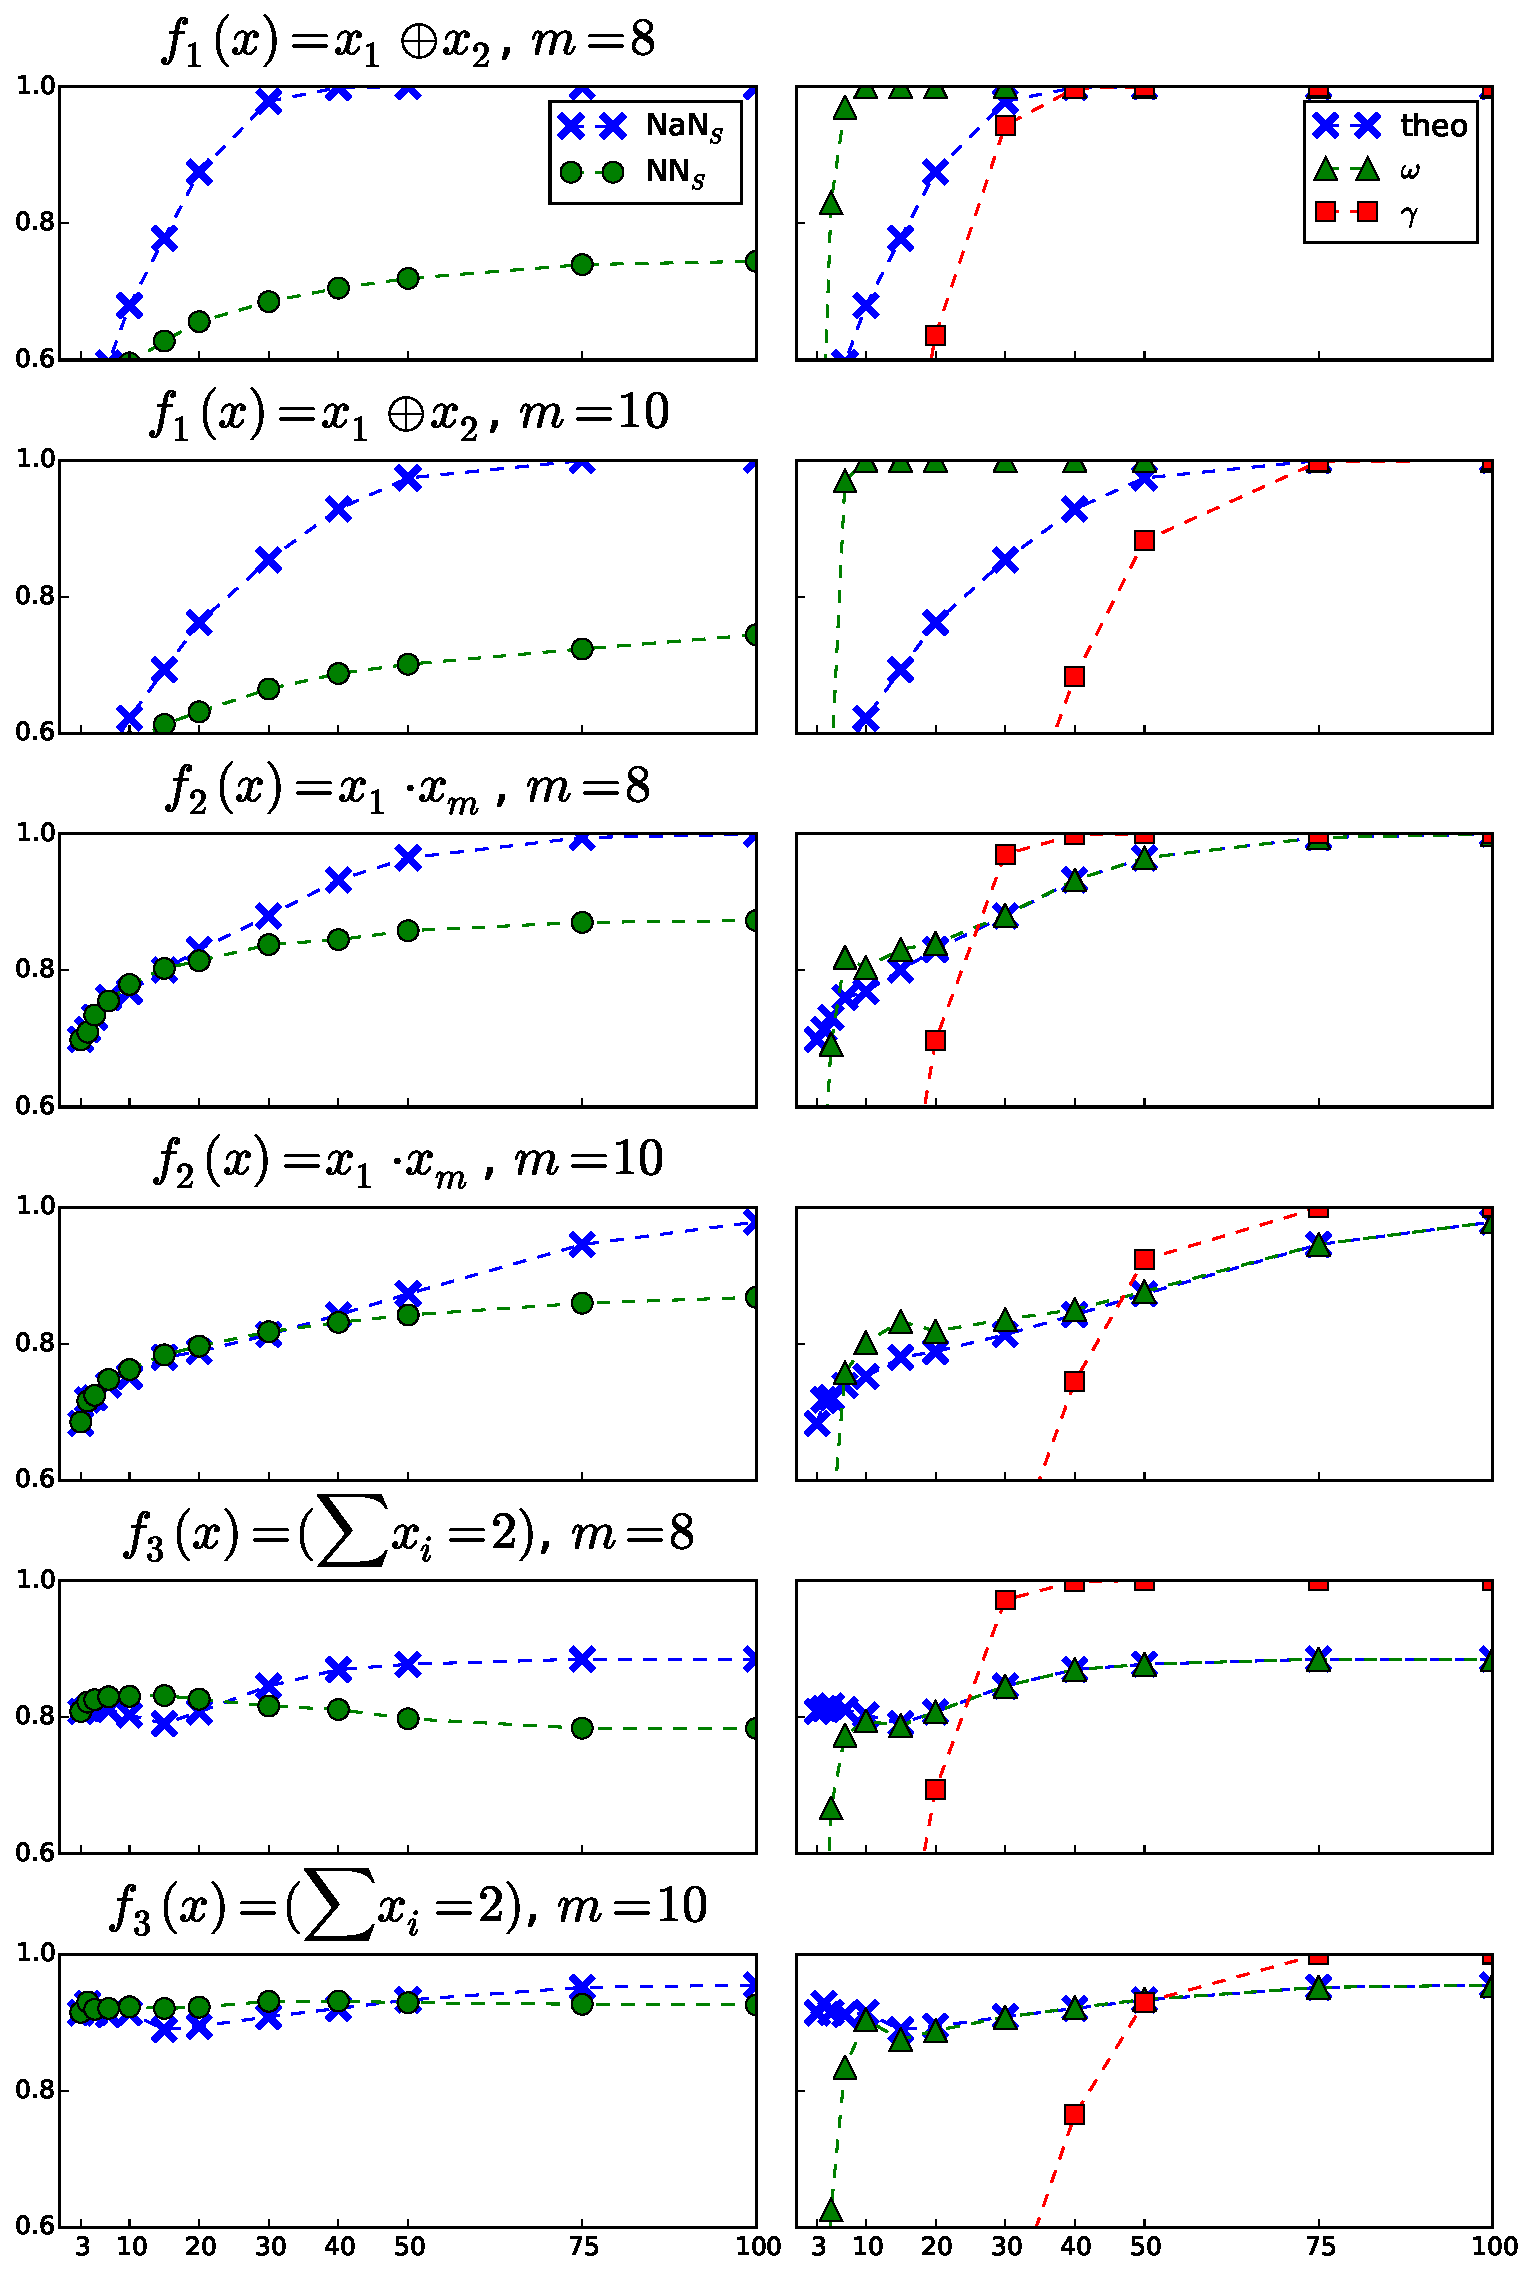
\includegraphics[width=\linewidth ]{figures/ecai_plots.pdf}
\end{figure}

Table \ref{TABLE_MONK} shows the same metrics for the Monk datasets and
also report the results of the Analogical Proportion Classifier (\textit{APC})
from \cite{MicBayDelJAIR2008}, which corresponds to algorithm
\ref{algo_extended} with $k=100$.

\begin{table}
\centering
\caption{Accuracies of the $\NaN$, APC and $\NN$ algorithms over the Monk datasets}
\label{TABLE_MONK}
\begin{tabular}{| c | c | c | c | c | c |}
\toprule
& $\NaN$  & APC & $\NN$  &  $\omega$ & $\gamma$ \\
\midrule
Monk 1 & .961 & .98 & .787 &   .961    &   1 \\
Monk 2 & .998 & 1 & .738 &    .996    &   1 \\
Monk 3 & .963 & .96 & .829 &   .963    &   1 \\
\bottomrule
\end{tabular}
\end{table}

\subsection{Comments and discussion}

The experiments shown in figure \ref{plots} allow us to draw interesting
conclusions about the behaviour of the $\NaN$ algorithm.  We can observe one of
the two cases:
\begin{itemize}
  \item either the analogical labels are always correctly
    predicted\footnote{Note that for small values of $|S|$, it seems that
      $\omega \neq 1$. This is due to the fact that for such small values, it
      is sometimes impossible to construct $A_E^Y(S)$, thus leading to a value
      of $\omega = 0$ (which will be averaged afterwards over the $100$
    experiments).}($\omega = 1$, i.e. there is no class noise) as it is the case for  $f_1$, $f(x) = x_m$ and
    (almost) for the Monk datasets~;
    \item or there is some class noise in $A_E^Y(S)$ ($\omega \neq 1$). In this
      case, we always observe that the $\NaN$ algorithm is outperformed by
      $\NN$ for small values of $|S|$, but eventually takes advantage once
      analogical prediction becomes more important than the nearest neighbour
      one, as we are going to see.
\end{itemize}

The theoretical accuracy seems to fit perfectly with the empirical accuracy of
the $\NaN$ algorithm, thus validating our theoretical study that led to
equation (\ref{ACCURACY_FORMULA})\footnote{The maximal difference we observed between the
theoretical accuracy and its actual value is of about $10^{-10}$.}.

An interesting observation is that the value of $\omega$ always converges to
that of the theoretical accuracy (and therefore to the actual accuracy) of
$\NaN$. This can be easily explained by paying attention to the value of
$\gamma$, the proportion of elements of $X$ that belong to $A_E^Y(S)$. We see
that in any setting, $\gamma$ converges to 1 as $|S|$ grows. This means that
when $|S|$ is big enough (but not necessarily \textit{that} big with respect to $X$), the
analogical extension of $S$ covers the whole universe $X$\footnote{Obviously,
the bigger the dimension $m$, the slower the convergence occurs.}: every
element $x$ is then its own nearest analogical neighbour and $\hat{x} =
\albl{x}$. It is therefore straightforward to see that in this case,
\begin{align*}
  \omega = P(\albl{x} = \dot{x} \given[\big] x \in A_E^*) &= P(\hat{x}
  = \dot{x} \given[\big] x \in A_E^*)\\
&= \acc(\NaN_S, A_E^*)
\end{align*}
When $\gamma = 1$, the only elements $x$ we want to classify belong to $A_E^*$
(otherwise they would be in $S$), so this last term exactly corresponds to the
accuracy of the classifier. Another way to see it is to observe that the first
term of equation (\ref{ACCURACY_FORMULA}) $\acc(\NN_{S}, A) \cdot \alpha$ is null
because $\alpha = 0$. Only the second term $\acc(\NN_{A_E^*}, B) \cdot (1 -
\alpha)$ is of importance, and its value corresponds to $\omega$. This
observation allows us to state that estimating the value of $\omega$ is
paramount to have a precise idea of the accuracy of an analogical classifier.
We will provide in the next subsection a method to accurately estimate this
quantity $\omega$ with the only help of the training set $S$.

Regarding the Monk datasets (Table \ref{TABLE_MONK}), we note that the
functional $\NaN$ approach (almost) achieves the same results as the somewhat
more complex algorithm described in Section \ref{EXTENDED_LEARNER}, and that
here again the analogical extension set covers the whole universe: this means
that a conservative approach would have been sufficient! Actually, this raises
the following question: why would we want to look for more than one analogical
neighbour when every element of the universe is already in $A_E^Y(S)$, and
therefore \textit{analogically linked} to those in $S$? Our experiments tend to
show that this becomes superfluous, provided that the training set is big
enough.

\subsection{Estimation of the prediction accuracy}

We have seen in the previous subsection that the value $\omega$ is that of the actual
accuracy of an analogical classifier when $S$ is big enough. This leads to the
following question: how can we get a precise estimation of this value $\omega$
? Answering this would allow us to have a very precise idea of the accuracy we
can expect from our classifier.

The method we propose for estimating $\omega$ only relies on the training set $S$
and is very simple: it consists of applying the conservative algorithm to all
the elements of $S$, and compute the fraction of these elements that have been
correctly classified. A small yet important modification to the algorithm needs
to be added: we only want to construct analogical proportions of the form $a :
b :: c : x$ where $a$, $b$, $c$ and $x$ are all distinct elements. Indeed, the
proportions $x : x :: x : x$ and $x' : x :: x' : x$ are always true, and the
solution label related to these proportions would bias the final majority vote
procedure in a significant way towards the real label $\dot{x}$.

We have applied this estimation protocol to all of the Boolean settings we have
considered, and it has shown to be very accurate. Figure \ref{omegaplots}
illustrates a few of these settings (already considered in Figure \ref{plots}).
\begin{figure}
  \caption{Values of $\omega$ and its estimation $\hat{\omega}$ for $f_1$, $f_2$ and $f_3$ in
  $\mathbb{B}^{10}$.}
\label{omegaplots}
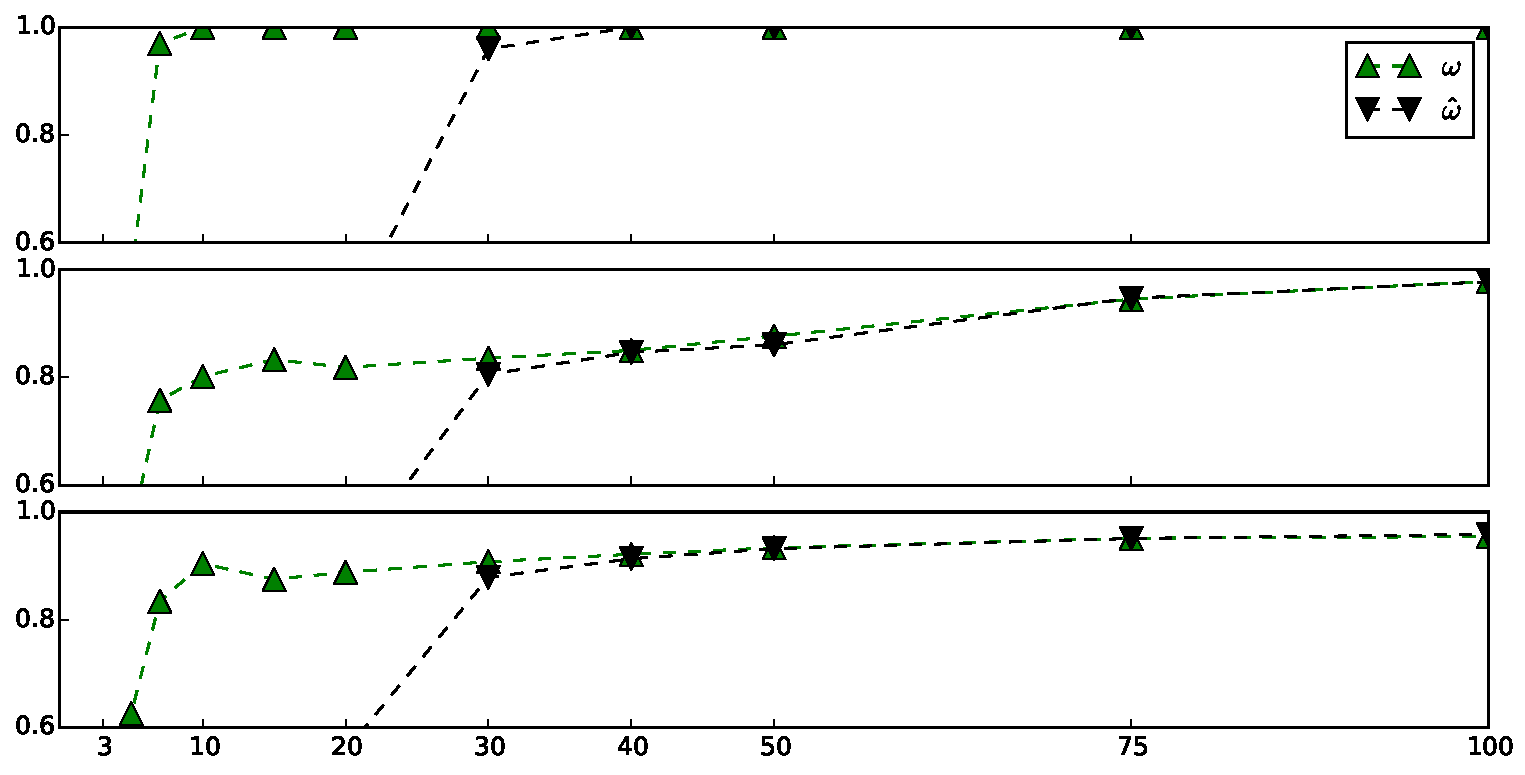
\includegraphics[width=\linewidth]{figures/ecai_estimation_omega.pdf}
\end{figure}
We can see that the estimation $\hat{\omega}$ converges to $\omega$ when $S$ is
big enough. For small values of $S$, this estimation is indeed imprecise as it
is difficult to find a lot a 3-tuples such that an analogical proportion holds
for every element.

\section{Conclusion}\label{conc}

In this paper, we have provided a  functional definition of analogical
learners.  Starting from this definition, we are in a position to prove an
analytic convergence result, similar to that of the nearest neighbour
algorithm. Obviously, this is not enough to conclude regarding the predictive
ability of analogy-based classifiers. We have also shown that their
VC\mbox{-}dimension is infinite.  It should not come as a surprise, as a very
particular case of analogical rule (when the analogical proportion is trivial)
is the $k$-NN rule.

This fact obviously has a consequence on the way we can
work to improve analogy-based classifier.  Indeed, learning by analogy is prone
to over-fitting and a relevant learning strategy should take this fact into
account.  Nevertheless, we have to keep in mind that the VC\mbox{-}dimension
alone is not a perfect marker of the quality of a machine learning algorithm,
especially when it comes
to practical implementation.

In terms of accuracy in a Boolean setting, we have found a strong link between
the accuracy of the $\NaN_S$ algorithm and that of the $\NN_S$ algorithm. At a
first glance, we can consider the $\NaN$ algorithm as a $\NN$ strategy on an
extended and noisy sample set: the analogical extension of $S$. In the end, we
have seen that this extended sample set covers the entire universe provided
that $S$ is big enough, simplifying and bringing back the accuracy of the
classifier to the value $\omega$ which corresponds to the  quality of the
analogical extension. We have also provided a method to accurately estimate the
value of $\omega$ that only relies on elements of the $S$, thus allowing
beforehand to have a precise idea of the accuracy of any analogical classifier
in a Boolean setting. Some important points remain to be investigated, such as:
\begin{itemize}
\item What can we expect in terms of speed convergence from an analogical
  learner? In other words, what is the minimum size needed from a sample set to
  get a fixed accuracy threshold?
\item If a clever learning strategy can (at least partially) overcome the
  problem of infinite VC\mbox{-}dimension, can we overcome the issue of the
  cubic complexity of analogical learners?
\item Leaving the field of classification, can we provide a clear strategy for
  transfer learning with analogy? Indeed, the central goal of transfer
    learning is to identify and exploit analogies between source and target
    domains \cite{Pan}.
\end{itemize}
\noindent
These points definitely constitute interesting challenges for future works.
Nevertheless, we have to remember that analogical reasoning brings its whole
power in the case where few data are available. If a lot of data are available,
it is very likely that we have elements similar to the one at hand and, in that
case, a $k$-NN style reasoning is natural. In the opposite case, when we only
have a few relevant cases at hand, applying analogical proportion-based
predictions appears to be a meaningful option.
